\setcounter{ex}{0}

% --- CÂU 1 ---
\begin{ex}
	Cho hàm số $y = f(x) = 2\cos x + 1$ có đồ thị trên đoạn $[-2\pi; 2\pi]$ như hình vẽ sau:
	\begin{center}
		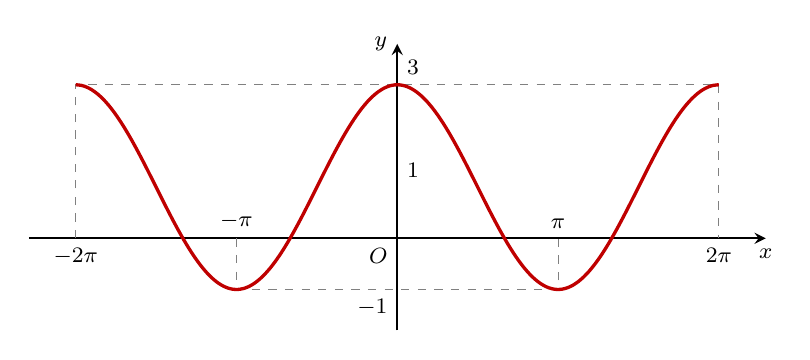
\begin{tikzpicture}[scale=0.65, font=\footnotesize, >=stealth]
			\draw[->, thick] (-7.2, 0) -- (7.2, 0) node[below] {$x$};
			\draw[->, thick] (0, -1.8) -- (0, 3.8) node[left] {$y$};
			\node[below left] at (0, 0) {$O$};
			\node[above right] at (0, 3) {$3$};
			\node[above right] at (0, 1) {$1$};
			\node[below left] at (0, -1) {$-1$};
			\node[below] at ({-2*pi}, 0) {$-2\pi$};
			\node[above] at ({-pi}, 0) {$-\pi$};
			\node[above] at ({pi}, 0) {$\pi$};
			\node[below] at ({2*pi}, 0) {$2\pi$};
			\draw[dashed, gray] ({-2*pi}, 0) -- ({-2*pi}, 3) -- ({2*pi}, 3) -- ({2*pi}, 0);
			\draw[dashed, gray] ({-pi}, 0) -- ({-pi}, -1) -- ({pi}, -1) -- ({pi}, 0);
			\draw[very thick, red!75!black, smooth, samples=120, domain={-2*pi}:{2*pi}] plot (\x, {2*cos(\x r) + 1});
		\end{tikzpicture}
	\end{center}
	Các mệnh đề sau đúng hay sai?
	\choiceTFt
	{\True Tập giá trị của hàm số $y = f(x)$ là đoạn $[-1; 3]$}
	{\True Hàm số đã cho là hàm số chẵn và tuần hoàn với chu kì $T = 2\pi$}
	{Hàm số đồng biến trên khoảng $(0; \pi)$}
	{\True Trên đoạn $[-2\pi; 2\pi]$, phương trình $f(x) = 0$ có đúng $4$ nghiệm phân biệt}
	\loigiai{
		\begin{itemchoice}
			\itemch \textbf{Đúng.} Vì $-1 \le \cos x \le 1, \forall x \in \mathbb{R}$ nên $-1 \le 2\cos x + 1 \le 3$. Vậy tập giá trị của hàm số là $[-1; 3]$.
			\itemch \textbf{Đúng.} Tập xác định $\mathscr{D} = \mathbb{R}$ đối xứng, với mọi $x \in \mathbb{R}$ ta có $f(-x) = 2\cos(-x) + 1 = 2\cos x + 1 = f(x)$ nên hàm số là hàm số chẵn và tuần hoàn với chu kì $T = 2\pi$.
			\itemch \textbf{Sai.} Dựa vào đồ thị, khi $x$ chạy từ $0$ đến $\pi$ thì đồ thị đi xuống (giá trị hàm số giảm từ $3$ xuống $-1$) nên hàm số nghịch biến trên khoảng $(0; \pi)$.
			\itemch \textbf{Đúng.} Đường thẳng $y = 0$ (trục hoành $Ox$) cắt đồ thị hàm số $y = f(x)$ trên đoạn $[-2\pi; 2\pi]$ tại đúng $4$ điểm phân biệt nên phương trình $f(x) = 0$ có đúng $4$ nghiệm phân biệt trên $[-2\pi; 2\pi]$.
		\end{itemchoice}
	}
\end{ex}

% --- CÂU 2 ---
\begin{ex}
	Cho hai hình bình hành $ABCD$ và $ABEF$ không đồng phẳng có tâm lần lượt là $O$ và $O'$. Khi đó:
	\choiceTFt
	{\True $OO' \parallel (ADF)$}
	{\True $OO' \parallel (BCE)$}
	{$OO' \parallel (ACE)$}
	{\True $OO' \parallel (CDFE)$}
	\loigiai{
		\begin{itemchoice}
			\itemch \textbf{Đúng.} Vì $O, O'$ lần lượt là trung điểm của $BD$ và $BF$ nên $OO'$ là đường trung bình của tam giác $BDF \implies OO' \parallel DF$. Mà $DF \subset (ADF)$ và $OO' \not\subset (ADF)$ nên $OO' \parallel (ADF)$.
			\itemch \textbf{Đúng.} Tương tự, $O, O'$ lần lượt là trung điểm của $AC$ và $AE$ nên $OO'$ là đường trung bình của tam giác $ACE \implies OO' \parallel CE$. Mà $CE \subset (BCE)$ và $OO' \not\subset (BCE)$ nên $OO' \parallel (BCE)$.
			\itemch \textbf{Sai.} Vì $O \in AC \subset (ACE)$ và $O' \in AE \subset (ACE)$ nên đường thẳng $OO'$ nằm trong mặt phẳng $(ACE)$ ($OO' \subset (ACE)$), không song song với $(ACE)$.
			\itemch \textbf{Đúng.} Ta có $OO' \parallel DF$, mà $DF \subset (CDFE)$ và $OO' \not\subset (CDFE)$ nên $OO' \parallel (CDFE)$.
		\end{itemchoice}
	}
\end{ex}

% --- CÂU 3 ---
\begin{ex}
	Cho cấp số cộng $(u_n)$ có số hạng đầu $u_1 = 3$, số hạng thứ tư $u_4 = 18$ và tổng $4$ số hạng đầu tiên bằng $42$. Các mệnh đề sau đúng hay sai?
	\choiceTFt
	{\True Công sai của cấp số cộng là $d = 5$}
	{Số hạng thứ ba của cấp số cộng là $u_3 = 12$}
	{\True Số các số hạng đầu tiên được xét trong tổng trên là $n = 4$}
	{\True Tổng của $10$ số hạng đầu tiên của cấp số cộng đó là $S_{10} = 255$}
	\loigiai{
		\begin{itemchoice}
			\itemch \textbf{Đúng.} Ta có $u_4 = u_1 + 3d \iff 18 = 3 + 3d \iff d = 5$.
			\itemch \textbf{Sai.} Số hạng thứ ba của cấp số cộng là $u_3 = u_1 + 2d = 3 + 2 \cdot 5 = 13 \ne 12$.
			\itemch \textbf{Đúng.} Kiểm tra tổng $4$ số hạng đầu tiên: $S_4 = \dfrac{4(u_1 + u_4)}{2} = 2(3 + 18) = 42$, do đó số các số hạng đầu tiên được xét trong tổng là $n = 4$.
			\itemch \textbf{Đúng.} Tổng của $10$ số hạng đầu tiên là:
			$$S_{10} = 10u_1 + \dfrac{10 \cdot 9}{2}d = 10 \cdot 3 + 45 \cdot 5 = 30 + 225 = 255.$$
		\end{itemchoice}
	}
\end{ex}

% --- CÂU 4 ---
\begin{ex}
	Cho phương trình lượng giác $\cos\left(x - \dfrac{\pi}{6}\right) = \dfrac{\sqrt{3}}{2}\ (*)$. Các mệnh đề sau đúng hay sai?
	\choiceTFt
	{\True Phương trình $(*)$ tương đương với $\cos\left(x - \dfrac{\pi}{6}\right) = \cos\dfrac{\pi}{6}$}
	{\True Phương trình có các họ nghiệm là $x = k2\pi$ và $x = \dfrac{\pi}{3} + k2\pi\ (k \in \mathbb{Z})$}
	{Trong khoảng $(-\pi; \pi)$, phương trình có tổng số $3$ nghiệm}
	{Nghiệm lớn nhất của phương trình trong khoảng $(0; 2\pi)$ là $\dfrac{5\pi}{3}$}
	\loigiai{
		\begin{itemchoice}
			\itemch \textbf{Đúng.} Vì $\cos\dfrac{\pi}{6} = \dfrac{\sqrt{3}}{2}$ nên phương trình $(*)$ tương đương với $\cos\left(x - \dfrac{\pi}{6}\right) = \cos\dfrac{\pi}{6}$.
			\itemch \textbf{Đúng.} Ta có:
			$$\cos\left(x - \dfrac{\pi}{6}\right) = \cos\dfrac{\pi}{6} \iff \hoac{x - \dfrac{\pi}{6} &= \dfrac{\pi}{6} + k2\pi \\ x - \dfrac{\pi}{6} &= -\dfrac{\pi}{6} + k2\pi} \iff \hoac{x &= \dfrac{\pi}{3} + k2\pi \\ x &= k2\pi}\ (k \in \mathbb{Z}).$$
			\itemch \textbf{Sai.} Xét trên khoảng $(-\pi; \pi)$:
			\begin{itemize}
				\item Họ nghiệm $x = k2\pi \in (-\pi; \pi) \iff k = 0 \implies x = 0$.
				\item Họ nghiệm $x = \dfrac{\pi}{3} + k2\pi \in (-\pi; \pi) \iff k = 0 \implies x = \dfrac{\pi}{3}$.
			\end{itemize}
			Vậy trong khoảng $(-\pi; \pi)$, phương trình chỉ có $2$ nghiệm là $x = 0$ và $x = \dfrac{\pi}{3}$.
			\itemch \textbf{Sai.} Trong khoảng $(0; 2\pi)$, phương trình chỉ có duy nhất một nghiệm là $x = \dfrac{\pi}{3}$.
		\end{itemchoice}
	}
\end{ex}
